\documentclass[12pt,a4paper]{report}

\usepackage[backend=biber, style=ieee]{biblatex}
\addbibresource{literature.bib}

\usepackage[utf8]{inputenc}
\usepackage[T1]{fontenc}
\usepackage[ngerman]{babel}
\usepackage{lmodern}
\usepackage{enumitem}
\usepackage{graphicx}
\usepackage{tabularx}
\usepackage{float}
\usepackage[onehalfspacing]{setspace}
\usepackage{microtype}
\usepackage{parskip}
\usepackage{minted}

\usepackage{xcolor}
\newcommand{\todo}[1]{\colorbox{red}{\textbf{TODO: #1}}\\}
\newcommand{\question}[1]{\colorbox{yellow}{\textbf{QUESTION: #1}}\\}
\newcommand{\xeno}[1]{\colorbox{pink}{\textbf{TODO XENO: #1}}\\}
\newcommand{\gideon}[1]{\colorbox{green}{\textbf{TODO GIDEON: #1}}\\}

\begin{document}

\tableofcontents
\newpage

\section{IntelliJ IDEA Companion}

Die Implementierung nutzt die von JetBrains bereitgestellten IntelliJ-Plugin-APIs, um sich direkt in den Entwicklungsablauf der IDE einzuklinken. Diese APIs ermöglichen es, Ereignisse wie einen erfolgreichen Code-Commit abzufangen, eigene Dialogfenster oder Benachrichtigungen anzuzeigen und auf gespeicherte Plugin-Einstellungen zuzugreifen. Dadurch kann das Yappi Companion-Plugin nahtlos in die bestehende IntelliJ-Oberfläche integriert werden, ohne den gewohnten Workflow der Entwickler zu unterbrechen.

Der IntelliJ Companion erweitert Yappi um die Möglichkeit, direkt aus der Entwicklungsumgebung heraus Feedback zu Code-Commits
zu erfassen. Ziel ist es, die Erfassung von Stimmungsdaten möglichst nahtlos in den Entwickler-Workflow zu integrieren, ohne den
Arbeitsfluss zu unterbrechen. Nach jedem erfolgreichen Commit in IntelliJ IDEA öffnet sich automatisch ein Dialogfenster, in dem
der Entwickler seine Stimmung sowie optional Notizen zum Commit angeben kann. Diese Daten werden anschliessend an Yappi übertragen
und dort gespeichert.

\subsection{Architektur und Integration}

Dia Abbildung~\ref{fig:intellij-system-diagram} zeigt den Aufbau des Yappi IntellJ IDEA Companion.

\begin{figure}[H]
\centering
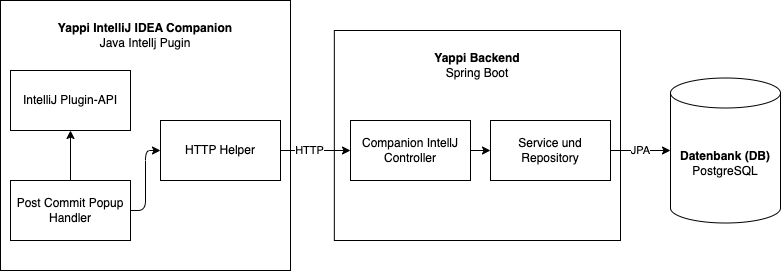
\includegraphics[width=0.95\textwidth]{../figures/intellij-system-diagram.drawio.png}
\caption{Architektur des IntelliJ IDEA Companion}
\label{fig:intellij-system-diagram}
\end{figure}

Die Implementierung basiert auf den IntelliJ-Plugin-APIs. Ein (\texttt{PostCommitPopupHandler}) registriert sich auf erfolgreiche
Commit-Events. Nach Bestätigung des Commits wird der Post-Commit-Dialog asynchron angezeigt, um die Haupt-UI nicht zu blockieren.
Der API-Key, der zur Authentifizierung gegenüber Yappi benötigt wird, wird über die Plugin-Einstellungen eingegeben und in einer
persistenten Komponente (\texttt{CompanionStorage}) gespeichert. Die Kommunikation mit dem Backend erfolgt über eine dedizierte
Hilfsklasse (\texttt{HttpHelper}), welche die Daten an den entsprechenden Endpoint überträgt.

\subsection{Speicherung der Einstellungen}

Damit sich die Companion App Authentifizieren kann muss ein gültiger API Key hinterlegt werden. Die Eingabe des API-Keys erfolgt
über den Menüpunkt Settings → Tools → Yappi Companion in IntelliJ. Die Abbildung~\ref{fig:intellij-settings} zeigt den 
entsprechenden Menupunkt.

\begin{figure}[H]
\centering
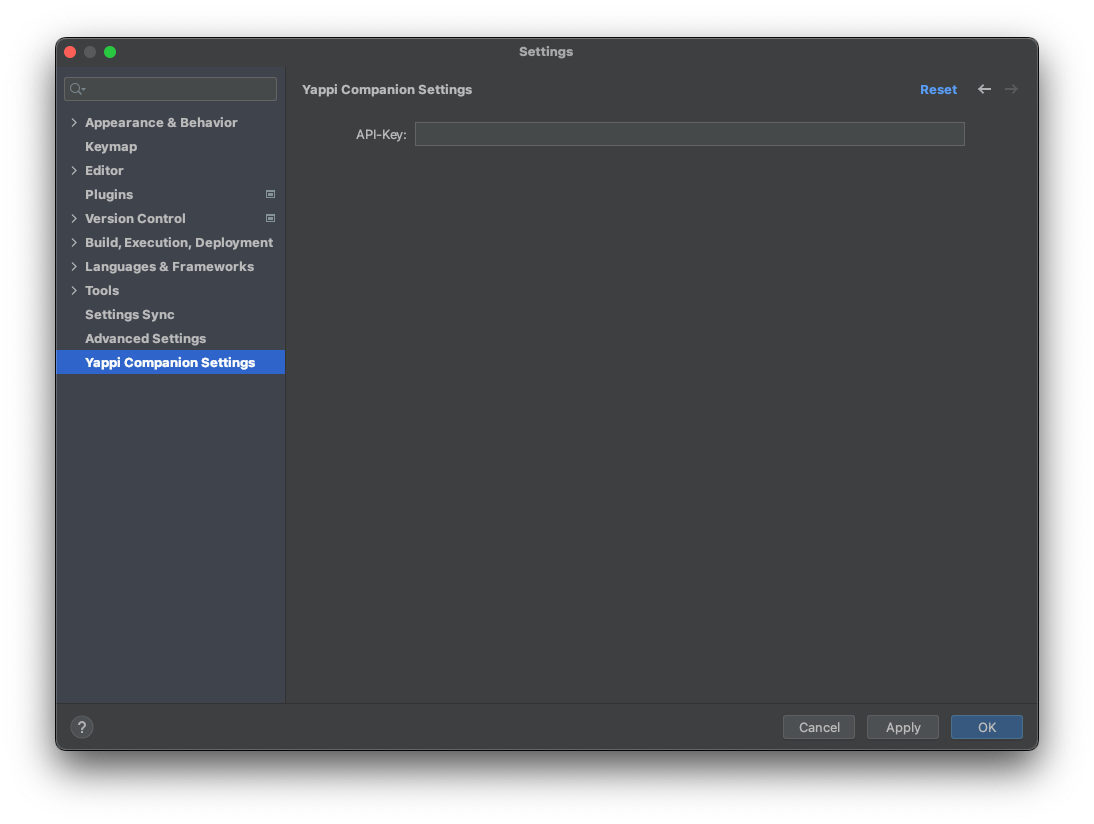
\includegraphics[width=0.95\textwidth]{../figures/intellij-settings.png}
\caption{Eingabe des API-Keys in den IntelliJ Companion-Einstellungen}
\label{fig:intellij-settings}
\end{figure}

Der Key wird in der Klasse \texttt{CompanionStorage} mithilfe der IntelliJ-Persistenzmechanismen gespeichert und beim nächsten
Start automatisch geladen.

\subsection{Post Commit Popup}

\begin{figure}[H]
\centering
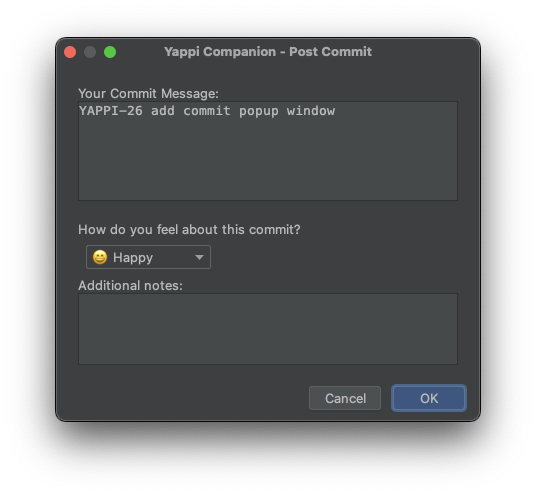
\includegraphics[width=0.95\textwidth]{../figures/intellij-post-commit.png}
\caption{Post-Commit-Dialog des IntelliJ Companions}
\label{fig:intellij-post-commit}
\end{figure}

\todo{neues design + text}
Die Benutzeroberfläche besteht aus:

\begin{itemize}
    \item Anzeige der Commit-Nachricht im oberen Bereich
    \item Auswahlfeld für die Stimmung mit vordefinierten Emojis (Happy, Neutral, Frustriert, Gestresst)
    \item Eingabefeld für zusätzliche Anmerkungen
\end{itemize}

Nach Bestätigung werden die Daten an Yappi gesendet, ohne dass weitere Aktionen des Nutzers nötig sind.

\subsection{Daten verarbeiten und Persistieren}

Die von der Companion App gesendeten Daten werden vom Backend empfangen und dort verarbeitet und anschliessend persistiert. In
Diesem Unterkapitel wird dieser Vorgang genauer beschrieben.

\subsubsection{Backend-Komponente}

Um die Daten im Backend zu emfangen wird ein neuer Controller erstellt, dieser heisst \texttt{IntellijCompanionController}. Der
folgende Endpoint wird von dem Controller bereitgestellt.

\begin{description}
  \item \texttt{POST /companion/commit} \\
        Erfasst Zufriedenheitsdaten inklusive Kontexinformationen nach einem Commit. \\
        \textbf{Antworten:} \texttt{200 OK}, \texttt{400 Bad Request}, \texttt{401 Unauthorized}.
\end{description}

Die empfangenen Daten werden überprüft und dann in der Datenbank persistiert.

\subsubsection{Datenbankerweiterung}

Die vom IntelliJ Companion übermittelten Zufriedenheitsdaten werden im Backend zusammen mit den zusätzlichen Kontextinformationen
persistiert. Während die eigentlichen Stimmungsdaten in der bestehenden Tabelle für Zufriedenheitsmessungen gespeichert werden,
wird für die Commit-bezogenen Zusatzinformationen eine separate, flexible Kontexttabelle angelegt. Diese Trennung erlaubt es, in
Zukunft weitere Arten von Kontextdaten ohne Änderungen Datenbankschama der Zufriedenheitsdaten zu integrieren.

Die Tabelle~\ref{tab:commit_context_schema} zeigt den Aufbau der neuen Kontexttabelle \texttt{commit_context}.

\todo{backend}

\printbibliography

\end{document}
